\subsection{Representa��o da plataforma sensor} 

A vers�o JProwler original implementa , como j� foi referido uma vis�o mais
monolitica da plataforma sensor sem a separa��o dos papeis de cada uma das
camadas da pilha de software de um \textit{mote}. Assim sendo a melhor forma de
estruturar um n� sensor � seguir um modelo de camadas, o que levou � separa��o
de cada um dos componentes que se encontravam consolidados numa �nica classe 
representativa de um n� sensor. Esta vis�o permitiu a separa��o de conceitos,
sendo consideradas apenas tr�s camadas: i) Camada MAC; ii) Camada de
Encaminhamento; iii) Camada de Aplica��o. Na figura \ref{fig:stack_components} �
poss�vel observar esta organiza��o. 

De forma tornar o n� sensor ainda mais
modular procurou-se mapear os componentes de um sensor num conjunto de classes,
tal como � apresentada na figura \ref{fig:stack_components}.
\begin{figure}[H]
\centering
\begin{tabular}{cccc|cccc}
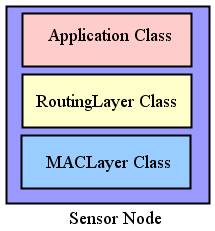
\includegraphics[height=5cm,width=4cm]{SensorNodeStack.png}
&  & & & & & & 
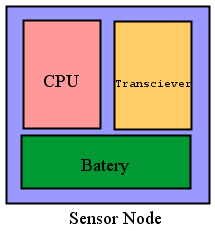
\includegraphics[height=5cm,width=4cm]{sensorNode_components.png}
\end{tabular}
\caption{Pilha de servi�os do sensor e  organiza��o por componentes}
\label{fig:stack_components}
\end{figure}
 
No que se refere � no��o de n� sensor tamb�m se pretende que este tenha um 
desenho bastante semelhante � arquitectura real. Para tal, o n� sensor �
modelado por componentes equivalentes � realidade f�sica. Isto �, existe um
componente \textit{CPU}, um componente \textit{Transciever} e um componente
\textit{Batery}. Este desenho permite que os dois primeiros componentes
interajam entre si e em particular com o terceiro para c�lculo do consumo
energ�tico. Assim, cada componente tem associado um conjunto de ac��es que s�o
da sua responsabilidade em que  cada uma consome um determinado valor energ�tico
(definido por parametriza��o do modelo de energia). 

Implementa��o de uma sem�ntica de \textit{timer} semelhante aos
\textit{temporizadores} de tinyOS
